\documentclass[12pt,a4paper]{article}
\usepackage[utf8]{inputenc}
\usepackage{amsmath}
\usepackage{amsfonts}
\usepackage{amssymb}

%bold Greek letters and other symbols
\usepackage{bm}
\usepackage{graphics}
\usepackage[T1]{fontenc}
\usepackage[english]{babel}
\usepackage{graphicx}
\usepackage[left=2.5cm,right=3.0cm,top=2.5cm,bottom=3cm]{geometry}
\usepackage{color}
%
\usepackage{makeidx}
\usepackage{shortvrb,latexsym}

\setlength{\parindent}{0pt}
%\renewcommand{\floatpagefraction}{.99}
%\renewcommand{\textfraction}{.01}
\def \oo {\bm{\omega}}
\def \curl {\bm{\nabla}\times}
\def \dive {\bm{\nabla}\cdot}
\newcommand{\bu}{\bm{u}}
\newcommand{\bv}{\bm{v}}
\newcommand{\rd}{\mathrm{d}}
\newcommand{\hx}{{\bf\hat{x}}}
\newcommand{\hy}{{\bf\hat{y}}}
\newcommand{\hz}{{\bf\hat{z}}}
\newcommand{\hr}{{\bf\hat{r}}}
\newcommand{\hn}{{\bf\hat{n}}}

\begin{document}

\begin{center}
2020-06-16
\end{center}
STOCKHOLMS UNIVERSITET\\
Meteorologiska Institutionen\\
Jonas Nycander, Dhrubaditra Mitra\\
\vspace{1cm}

\begin{center}
{\bf\large Exam in Fluid mechanics (MO5001)}\\
\end{center}

Write the solution of each problem on a separate paper, and write your identification number on every paper.\\

{\bf Allowed aids:} calculator, sheet with vector analysis relations.\\

{\bf Grading:} A 90-100\%, B 80-89\%, C 65-79\%, D 55-64\%, E 50-54\%, Fx 45-49\%, F 0-44\% \\
\vspace{0.5cm}

\begin{enumerate}

\item \label{prb1} Answer the following short questions. You just need to write the final answer. Each question is worth 3 points. 
  \begin{enumerate}
  \item A vector field, $\bu$, with components $u_x$, $u_y$ and $u_z$,  as a function  of
    space (described by $x$, $y$, and $z$ coordinates )
    is give by the following expression
    \begin{eqnarray}
      u_x &=& \alpha [2x + \cos(y) + 5z^3 ] \nonumber \\
      u_y &=& \alpha[ e^{-x} - y + \sin(y) ] \nonumber \\
      u_z &=& \alpha[ \sin(x) + \cos(y) -z ]
    \end{eqnarray}
   Let $\oo = \curl \bu$. Calculate $\dive \oo$. 
 \item A velocity field $\bu$ in two-dimensions $(x,y)$ is given by the following expression
   \begin{subequations}
     \begin{align}
     u_x &= x \\
     u_y &= Sx -y   \/.
     \end{align}
     \label{eq:uu}
   \end{subequations}
   Calculate the gradient matrix $ G_{\alpha\beta} \equiv \partial_{\beta}u_{\alpha}$, where
   $\partial_{\beta}$ denote spatial derivative, as a function of $x$ and $y$. Is this velocity
   field incompressible ? 
 \item From Eq.~\ref{eq:uu}  calculate vorticity and rate-of-strain as a function of
   space coordinates, $x,y$.
 \item Which of the following are true ? (More than one may be true. )
   Viscosity of a Newtonian fluid is
   \begin{enumerate}
   \item a scalar.
   \item can be described by two scalar quantities.
     \item is a fourth rank tensor. 
    \end{enumerate}
 \item Organize the images in figure~\label{fig:images} in
   sequence of increasing Reynolds number. 
   \begin{figure}
     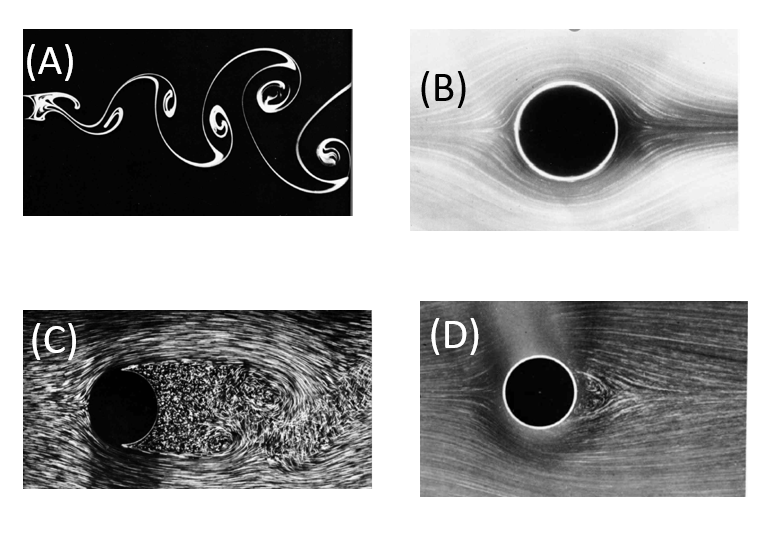
\includegraphics{exam2021_image.PNG}
     \caption{\label{fig:images} Organize these images in sequence of increasing Reynolds number} 
   \end{figure}
   \end{enumerate}
\item ({\bf 5 pt})
  The figure~\ref{dam} sketches a dam wall. The height of the water in the
  reservoir is $h$. What is the net \textit{horizontal} force acting on the wall of the 
dam ? 
  \begin{figure}[h!]
    \begin{center}
    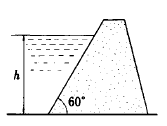
\includegraphics[width=0.4\linewidth]{dam.png}
    \caption{ Sketch of dam \label{dam}}
    \end{center}
  \end{figure}

\item ({\bf 5 pt}) A thin horizontal disc of radius $R$ is located in a cylindrical cavity filled with oil
  with dynamic viscosity $\mu$. The clearence between the disc and the horizontal planes of
  the cavity is equal to $h$. Using lubrication approximation calculate the power
  necessary to rotate the disc with a constant angular velocity $\omega$. Ignore the end
  effects.  
  %===================================================================

%====================================================================
\end{enumerate}
\end{document}
